% Bitácora 2: Guía de estudio de las integrales de camino
% Se incluye desde main.tex con \input; no compilar este archivo solo.

\part{Bitácora 2: Guía de estudio de las integrales de camino}
\setcounter{section}{0}
\begin{center}\normalsize Plan de estudio de 12 horas con NotebookLM. 27 de septiembre de 2026.\end{center}


\section{Datos de la sesión}

\begin{itemize}
    \item \textbf{Tarea.} Con ayuda de la IA (NotebookLM), elaborar una guía para estudiar las integrales de camino desde lo más básico, en unas 12 horas, indicando en cada paso qué fuente usar y cómo usarla.
    \item \textbf{IA principal:} NotebookLM, sobre un cuaderno propio con las fuentes del profesor pasadas a Markdown (\href{https://notebook.google.com/notebook/379b66c2-c80a-4d9d-8339-739a3fd3054b}{enlace al cuaderno}).
    \item \textbf{IA auditora:} Claude (Opus 5.5): preparación de las fuentes y revisión de la guía.
    \item \textbf{Roles:} prompts y línea principal: Valentina; cuestionador: Sebastián; revisor/verificador: Luis.
\end{itemize}

%======================================================================
\section{Cómo usar esta guía}

\subsection{Objetivo}

Al terminar las 12 horas, el estudiante debe poder, sin ayuda:
\begin{enumerate}[label=(O\arabic*)]
    \item explicar qué significa ``sumar sobre todos los caminos'' y por qué el peso de cada camino es $e^{iS/\hbar}$;
    \item deducir la integral de camino a partir de la ecuación de Schrödinger (y viceversa);
    \item calcular el propagador de la partícula libre y del oscilador armónico;
    \item explicar por qué, cuando $\hbar\to0$, solo sobrevive la trayectoria clásica, es decir, de dónde sale la mecánica de Newton;
    \item reconocer dónde se usa hoy el formalismo: mecánica estadística, cálculo numérico, fases topológicas y teoría de campos.
\end{enumerate}

\subsection{Punto de partida}

\textbf{Se supone conocido:} la segunda ley de Newton, el cálculo en varias variables, la integral gaussiana real $\int e^{-ax^2}\dd x=\sqrt{\pi/a}$, la ecuación de Schrödinger y la notación de Dirac de un primer curso de cuántica.

\textbf{No se supone conocido} (se aprende aquí): la mecánica lagrangiana, el cálculo variacional, las integrales gaussianas complejas y el propagador como núcleo integral.

\subsection{Qué cubre y qué no}

Cubre la mecánica cuántica no relativista de una partícula en una dimensión, con $L=\tfrac12m\dot x^2-V(x)$, y al final el acoplamiento a un campo electromagnético. No cubre los fermiones (variables de Grassmann) ni la teoría rigurosa de la medida; la teoría de campos solo se asoma en la última sesión.

\subsection{Método de cada sesión}

Cada sesión dura una hora y sigue siempre los mismos cinco pasos:
\begin{enumerate}
    \item \textbf{Idea clave} (5 min): leer el resumen de esta guía.
    \item \textbf{Leer} (25 min): la sección indicada de la fuente principal. La fuente de apoyo es para cuando algo no se entienda.
    \item \textbf{Preguntar a NotebookLM} (10 min): usar el prompt propuesto. Todos piden citar la fuente y el número de ecuación, para poder comprobar la respuesta en el texto original. \emph{Nunca se acepta una ecuación de la IA sin encontrarla en la fuente.}
    \item \textbf{Ejercicio} (15 min): hacerlo en papel, sin mirar.
    \item \textbf{Autoevaluación} (5 min): si no se puede responder a la pregunta de control, se repite el paso 2 antes de pasar a la sesión siguiente.
\end{enumerate}

\subsection{Criterio de cierre}

La guía se da por completada cuando se pueden hacer de memoria los tres ejercicios marcados con $\bigstar$ (sesiones 3, 4 y 7) y se aprueba la autoevaluación final (sección~\ref{sec:final}).

%======================================================================
\section{Mapa del tema}

La ruta va de lo clásico a lo cuántico y vuelve a lo clásico:
\[
\underbrace{F=ma}_{\text{S1}}\;\to\;\underbrace{S=\!\int\! L\,\dd t}_{\text{S1}}\;\to\;
\underbrace{\text{amplitudes}}_{\text{S2}}\;\to\;
\underbrace{\textstyle\int\mathcal Dx\,e^{iS/\hbar}}_{\text{S3--5}}
\]
\[
\to\;
\underbrace{\text{oscilador}}_{\text{S6}}\;\to\;
\underbrace{\hbar\to0:\ F=ma}_{\text{S7}}\;\to\;
\underbrace{\text{aplicaciones}}_{\text{S8--12}}
\]

\begin{center}
\begin{tabular}{@{}c p{5.4cm} l l@{}}
\toprule
Sesión & Tema & Fuente principal & Apoyo \\
\midrule
1 & De las fuerzas a la acción & \F{02} cap.~1 & \F{06} \S1 \\
2 & Amplitudes y propagador & \F{06} \S2, \S9--10 & \F{12} \S3.1 \\
3 & Construcción de la integral de camino $\bigstar$ & \F{01} \S2.1 & \F{11} \S2.3, \F{09} \S2.1 \\
4 & Gaussianas y partícula libre $\bigstar$ & \F{11} ap.~A, \F{01} \S2.2 & \F{06} \S3--5, \F{09} \S2.2 \\
5 & Equivalencia con Schrödinger & \F{11} \S2.4--2.5 & \F{06} \S6 \\
6 & Oscilador armónico & \F{01} \S2.2 & \F{09} \S2.3--2.4, \F{13} \S1.3 \\
7 & Límite clásico y semiclásico $\bigstar$ & \F{01} \S3 & \F{13} \S3.1, \F{11} \S3 \\
8 & Tiempo imaginario y estadística & \F{13} \S2.2 & \F{01} \S5, \F{12} \S3.4 \\
9 & Cálculo numérico (PIMC) & \F{10} \S2 & \F{02} cap.~1 (numérico) \\
10 & Campo electromagnético y topología & \F{01} \S4 & \F{13} cap.~5, \F{06} \S18 \\
11 & Efecto túnel e instantones & \F{13} cap.~4 & \F{01} \S8 \\
12 & Átomo de hidrógeno y teoría de campos & \F{03} \S III.5, \F{07} \S3--4 & \F{04}, \F{05} \\
\bottomrule
\end{tabular}
\end{center}

%======================================================================
\section{Las fuentes y para qué sirve cada una}

Todas están en el cuaderno propio de NotebookLM. La numeración \F{01}--\F{15} es la que se usa en toda la guía.

\begin{longtable}{@{}l p{5.2cm} p{2.6cm} p{5.2cm}@{}}
\toprule
 & Obra & Autor, año & Usarla para \\
\midrule
\endhead
\F{01} & \textit{Path Integral Methods and Applications} & R.~MacKenzie, 2000 & \textbf{Texto base.} Claro, corto y cubre casi todo el plan. \\
\F{02} & \textit{Path Integrals in Quantum Physics} & R.~Rosenfelder, 2017 & Curso completo; el cap.~1 para el principio de acción y como consulta. \\
\F{03} & \textit{An Introduction into the Feynman Path Integral} & C.~Grosche, 1993 & Derivación cuidadosa (orden de operadores) y ejemplos resueltos. \\
\F{04} & \textit{Path integral of the hydrogen atom\dots} & K.~Fujikawa, 1996 & Solo sesión 12 (avanzado). \\
\F{05} & \textit{How to solve path integrals in QM} & C.~Grosche, F.~Steiner, 1995 & Catálogo de soluciones exactas (avanzado). \\
\F{06} & \textit{Feynman Path Integral: Formulation of Quantum Dynamics} & M.~S.~Suzuki, 2021 & \textbf{El más intuitivo.} Diagramas de fasores, rendija, Mathematica. \\
\F{07} & \textit{Introduction to path-integral QFT -- A toolbox} & R.~Köberle, 2021 & Integrales gaussianas y puente a teoría de campos. \\
\F{08} & \textit{Path Integrals in QM, Statistics, Polymer Physics\dots} & H.~Kleinert, 2009 & Enciclopedia; solo para consulta puntual. \\
\F{09} & \textit{Path Integrals --- Elementary Properties\dots} (cap.~2 de \F{08}) & H.~Kleinert & Cálculos exactos con todo detalle. \\
\F{10} & \textit{Path Integral Monte Carlo and Hydrogen bond} & T.~Saporiti, 2020 & Cálculo numérico (sesión 9). \\
\F{11} & \textit{Path integrals in QM, Semiclassical approximation} & T.~Saporiti, 2022 & \textbf{El más corto} (8 págs.). Ideal para empezar a derivar. \\
\F{12} & \textit{Lecture 3: Path integrals in QM} & J.~Zinn-Justin & Enfoque estadístico y funcional generatriz. \\
\F{13} & \textit{The Path Integral approach to QM} & R.~Rattazzi, 2009 & Notas de curso: determinantes, euclídeo, semiclásico, instantones. \\
\F{14} & \textit{Exact path integral treatment of the hydrogen atom} & F.~Steiner, 1984 & Histórico (sesión 12). \\
\F{15} & \textit{Quantum Mechanics and Path Integrals} & R.~P.~Feynman, A.~R.~Hibbs & El clásico; caps.~1--3 como lectura motivacional. \\
\bottomrule
\end{longtable}

\textbf{Si solo hay tiempo para tres:} \F{01} (base), \F{06} (intuición) y \F{11} (derivación compacta).

%======================================================================
\section{Plan de estudio: 12 sesiones}

%----------------------------------------------------------------------
\sesion{1 --- De las fuerzas a la acción}{1 h}

\campo{Idea clave}
La mecánica de Newton se puede reformular sin fuerzas: de todas las trayectorias $x(t)$ que van de $(x_a,t_a)$ a $(x_b,t_b)$, la real es la que hace \emph{estacionaria} la acción
\[
S[x]=\int_{t_a}^{t_b}L(x,\dot x)\,\dd t,\qquad L=T-V=\tfrac12m\dot x^2-V(x).
\]
Pedir $\delta S=0$ da la ecuación de Euler--Lagrange $\frac{\dd}{\dd t}\frac{\partial L}{\partial\dot x}-\frac{\partial L}{\partial x}=0$, que para este $L$ es exactamente $m\ddot x=-V'(x)=F$. Esta es la pieza que la cuántica va a ``explicar'' en la sesión 7.

\campo{Leer}
\F{02}, cap.~1, sección \textit{Action Principle and Sum over all Paths}. Apoyo: \F{06} \S1 (repasa la ecuación de Lagrange); \F{01} \S1 (\textit{Motivation}).

\campo{Preguntar a NotebookLM}
\begin{prompt}
Usando \F{02} y \F{06}, explica paso a paso cómo se pasa de la segunda ley de Newton al principio de mínima acción. Muestra la deducción de Euler--Lagrange e indica en qué ecuación de cada fuente aparece.
\end{prompt}

\campo{Ejercicio}
Calcular la acción clásica $S_{\text{cl}}$ para (a) la partícula libre, $S_{\text{cl}}=m(x_b-x_a)^2/2T$; (b) el oscilador armónico. Comprobar en (a) que $\partial S_{\text{cl}}/\partial x_b=p_b$.

\campo{Autoevaluación}
¿Por qué se dice ``acción estacionaria'' y no ``mínima''? (Pista: oscilador con $T>\pi/\omega$.)

%----------------------------------------------------------------------
\sesion{2 --- Amplitudes y propagador}{1 h}

\campo{Idea clave}
En cuántica no hay trayectoria: hay \emph{amplitudes}. La amplitud de ir de $x_a$ a $x_b$ en un tiempo $T$ es el propagador
\[
K(x_b,T;x_a,0)=\langle x_b|e^{-i\hat HT/\hbar}|x_a\rangle,\qquad
\psi(x_b,T)=\int K(x_b,T;x_a,0)\,\psi(x_a,0)\,\dd x_a .
\]
Dos reglas bastan para todo lo demás: (i) si hay varias alternativas, las amplitudes \emph{se suman}; (ii) si un proceso pasa por un punto intermedio, las amplitudes \emph{se multiplican} y se integra sobre ese punto:
$K(x_c,t_2;x_a,0)=\int K(x_c,t_2;x_b,t_1)K(x_b,t_1;x_a,0)\,\dd x_b$.

\campo{Leer}
\F{06} \S2 (\textit{Propagator}) y \S9--10 (rendija y diagrama de fasores: se ve cómo al sumar cada vez más caminos aparece el patrón de difracción). Apoyo: \F{12} \S3.1; \F{15} cap.~1 (la doble rendija contada por Feynman).

\campo{Preguntar a NotebookLM}
\begin{prompt}
Según \F{06}, ¿cómo se obtiene el patrón de una rendija sumando fasores de 2, 6 y 36 caminos? Explica qué representa la longitud y el ángulo de cada fasor.
\end{prompt}

\campo{Ejercicio}
Escribir la regla de composición para tres tiempos intermedios y ver que, repetida $N$ veces, ``llena'' el intervalo de puntos intermedios. Esa es la idea de la sesión 3.

\campo{Autoevaluación}
¿Qué magnitud física da $|K|^2$? ¿Qué unidades tiene $K$?

%----------------------------------------------------------------------
\sesion{3 --- Construcción de la integral de camino $\bigstar$}{1 h}

\campo{Idea clave}
Se parte el tiempo en $N$ pasos de duración $\varepsilon=T/N$ y en cada paso se inserta la identidad $\int\dd x_k\,|x_k\rangle\langle x_k|$. Para un paso corto vale $e^{-i\varepsilon(\hat T+\hat V)/\hbar}\approx e^{-i\varepsilon\hat T/\hbar}e^{-i\varepsilon\hat V/\hbar}$ (fórmula de Trotter) y la amplitud de un paso es
\[
\langle x_{k+1}|e^{-i\varepsilon\hat H/\hbar}|x_k\rangle\approx\sqrt{\frac{m}{2\pi i\hbar\varepsilon}}\;
\exp\!\Big\{\frac{i\varepsilon}{\hbar}\Big[\frac m2\Big(\frac{x_{k+1}-x_k}{\varepsilon}\Big)^2-V(x_k)\Big]\Big\}.
\]
El exponente es $i/\hbar$ por la acción de un tramo recto. Multiplicando los $N$ pasos:
\[
K(x_b,T;x_a,0)=\lim_{N\to\infty}\Big(\frac{m}{2\pi i\hbar\varepsilon}\Big)^{N/2}\int\prod_{k=1}^{N-1}\dd x_k\;e^{iS_N/\hbar}\;\equiv\;\int\mathcal Dx\;e^{iS[x]/\hbar}.
\]
Cada elección de $x_1,\dots,x_{N-1}$ es un camino en zigzag; integrar sobre todas es ``sumar sobre todos los caminos'', cada uno con el mismo módulo y con fase $S/\hbar$.

\campo{Leer}
\F{01} \S2.1 (\textit{General discussion}). Apoyo: \F{11} \S2.3 (\textit{Feynman's solution}), versión compacta; \F{09} \S2.1, versión detallada; \F{03} \S II.1--II.2, para ver por qué importa el orden de los operadores.

\campo{Preguntar a NotebookLM}
\begin{prompt}
Compara la derivación de la integral de camino en \F{01}, \F{11} y \F{03}. ¿En qué paso usa cada una la fórmula de Trotter y cómo tratan el prefactor $(m/2\pi i\hbar\varepsilon)^{N/2}$? Señala cualquier diferencia de convención.
\end{prompt}

\campo{Ejercicio $\bigstar$}
Reproducir la derivación completa en una hoja sin mirar, incluida la integral sobre los momentos intermedios.

\campo{Autoevaluación}
¿Qué significa $\mathcal Dx$? ¿Por qué no es una integral ``normal''?

%----------------------------------------------------------------------
\sesion{4 --- Integrales gaussianas y partícula libre $\bigstar$}{1 h}

\campo{Idea clave}
Casi todo lo que se calcula exactamente sale de una sola fórmula, la integral gaussiana, válida también para $a$ imaginario puro si se da a $a$ una parte real positiva infinitesimal:
\[
\int_{-\infty}^{\infty}e^{-ax^2+bx}\,\dd x=\sqrt{\frac{\pi}{a}}\;e^{b^2/4a}.
\]

\textbf{Ejemplo resuelto: el propagador libre.} Con $V=0$, dos pasos de duraciones $\tau_1,\tau_2$ se combinan así:
\[
\int\dd y\;e^{\frac{im}{2\hbar}\left[\frac{(x-y)^2}{\tau_1}+\frac{(y-z)^2}{\tau_2}\right]}
=\sqrt{\frac{2\pi i\hbar}{m}\frac{\tau_1\tau_2}{\tau_1+\tau_2}}\;e^{\frac{im}{2\hbar}\frac{(x-z)^2}{\tau_1+\tau_2}} .
\]
Los prefactores también se combinan: $\sqrt{\tfrac{m}{2\pi i\hbar\tau_1}}\sqrt{\tfrac{m}{2\pi i\hbar\tau_2}}\sqrt{\tfrac{2\pi i\hbar\tau_1\tau_2}{m(\tau_1+\tau_2)}}=\sqrt{\tfrac{m}{2\pi i\hbar(\tau_1+\tau_2)}}$. Por inducción, las $N-1$ integrales dan, para cualquier $N$,
\[
\boxed{K_0(x_b,T;x_a,0)=\sqrt{\frac{m}{2\pi i\hbar T}}\;\exp\!\Big[\frac{im(x_b-x_a)^2}{2\hbar T}\Big]=\sqrt{\frac{m}{2\pi i\hbar T}}\;e^{iS_{\text{cl}}/\hbar}.}
\]

\textbf{Comprobaciones} (hacerlas siempre):
\begin{itemize}
    \item \emph{Dimensiones:} $[m/\hbar T]=\mathrm{m}^{-2}$, así que $[K]=\mathrm{m}^{-1}$, lo que necesita $\psi(x_b)=\int K\psi\,\dd x_a$.
    \item \emph{Límite $T\to0$:} gaussiana de anchura $\sqrt{\hbar T/m}\to0$ y área 1, es decir, $K\to\delta(x_b-x_a)$.
    \item \emph{Otro camino:} insertando autoestados de momento, $K_0=\int\frac{\dd p}{2\pi\hbar}e^{ip(x_b-x_a)/\hbar-ip^2T/2m\hbar}$, que es una sola gaussiana y da lo mismo.
\end{itemize}

\campo{Leer}
\F{11} ap.~A (\textit{Gaussian integral}) y \F{01} \S2.2 (\textit{Free particle}). Apoyo: \F{06} \S3--5; \F{09} \S2.2; \F{07} \S2 para las gaussianas en muchas variables.

\campo{Preguntar a NotebookLM}
\begin{prompt}
Calcula el propagador de la partícula libre como en \F{01} \S2.2. Después verifica que tiende a $\delta(x_b-x_a)$ cuando $T\to0$. Cita la ecuación de la fuente en cada paso.
\end{prompt}
(Comparar la respuesta con el ejemplo resuelto de arriba.)

\campo{Ejercicio $\bigstar$}
Rehacer el ejemplo resuelto y el recálculo por momentos sin mirar.

\campo{Autoevaluación}
¿Por qué el resultado no depende de $N$ en este caso? ¿Pasaría lo mismo con $V\neq0$?

%----------------------------------------------------------------------
\sesion{5 --- Equivalencia con la ecuación de Schrödinger}{1 h}

\campo{Idea clave}
La integral de camino no es una teoría nueva: es la misma cuántica escrita de otra forma. Si se aplica un solo paso corto a $\psi$ y se desarrolla en $\varepsilon$, se recupera
$i\hbar\,\partial_t\psi=-\tfrac{\hbar^2}{2m}\partial_x^2\psi+V\psi$.
Al revés, de Schrödinger se llega a la integral de camino (sesión 3).

\campo{Leer}
\F{11} \S2.4 (\textit{Schrödinger implies Feynman}) y \S2.5 (\textit{Feynman implies Schrödinger}). Apoyo: \F{06} \S6.

\campo{Preguntar a NotebookLM}
\begin{prompt}
Según \F{11} \S2.5, ¿cómo se deduce la ecuación de Schrödinger a partir de un paso de la integral de camino? ¿Qué términos del desarrollo en $\varepsilon$ se conservan y por qué el término en $\eta=x-y$ contribuye a orden $\varepsilon$?
\end{prompt}

\campo{Ejercicio}
Comprobar directamente que $K_0$ de la sesión 4 cumple la ecuación de Schrödinger libre: con $K_0=A\,T^{-1/2}e^{imx^2/2\hbar T}$, los dos lados valen $\left(-\frac{i\hbar}{2T}+\frac{mx^2}{2T^2}\right)K_0$.

\campo{Autoevaluación}
¿Por qué, en un paso corto, los caminos relevantes tienen $|x_{k+1}-x_k|\sim\sqrt{\varepsilon}$ y no $\sim\varepsilon$? ¿Qué dice eso de la ``velocidad'' de los caminos?

%----------------------------------------------------------------------
\sesion{6 --- Oscilador armónico y fluctuaciones}{1 h}

\campo{Idea clave}
Si el lagrangiano es cuadrático, se escribe cada camino como $x=x_{\text{cl}}+\eta$ con $\eta(0)=\eta(T)=0$. La acción se separa en $S[x_{\text{cl}}]+S[\eta]$ y queda
\[
K=F(T)\,e^{iS_{\text{cl}}/\hbar},
\]
donde $F(T)$ no depende de los extremos y se calcula como un determinante (de ahí la fórmula de Gelfand--Yaglom). Para el oscilador:
\[
K_\omega=\sqrt{\frac{m\omega}{2\pi i\hbar\sin\omega T}}\exp\Big\{\frac{im\omega}{2\hbar\sin\omega T}\big[(x_a^2+x_b^2)\cos\omega T-2x_ax_b\big]\Big\}.
\]

\campo{Leer}
\F{01} \S2.2 (\textit{Harmonic oscillator}). Apoyo: \F{09} \S2.3--2.4 (cálculo exacto y Gelfand--Yaglom); \F{13} \S1.3 (\textit{Path integrals as determinants}); \F{12} \S3.5.2.

\campo{Preguntar a NotebookLM}
\begin{prompt}
Según \F{01} y \F{09}, ¿cómo se calcula el factor de fluctuación $F(T)$ del oscilador armónico? Explica qué pasa cuando $\omega T=n\pi$ y cita las ecuaciones.
\end{prompt}

\campo{Ejercicio}
Tomar $\omega\to0$ en $K_\omega$ y comprobar que se recupera $K_0$.

\campo{Autoevaluación}
¿Qué ocurre físicamente en $\omega T=\pi$ (todas las trayectorias clásicas se reenfocan) y por qué el prefactor diverge ahí?

%----------------------------------------------------------------------
\sesion{7 --- El límite clásico: de vuelta a $F=ma$ $\bigstar$}{1 h}

\campo{Idea clave}
Cuando $S\gg\hbar$, la fase $e^{iS/\hbar}$ oscila muy rápido de un camino a otro y las contribuciones se cancelan, \emph{excepto} cerca del camino donde $S$ es estacionaria, porque ahí caminos vecinos tienen casi la misma fase. Ese camino cumple $\delta S=0$, es decir, $m\ddot x=F$. \textbf{El principio de mínima acción de la sesión 1 sale de la cuántica.} Desarrollando hasta segundo orden alrededor de $x_{\text{cl}}$ se obtiene la aproximación semiclásica (Van Vleck):
\[
K\approx\sqrt{\frac{1}{2\pi i\hbar}\left|-\frac{\partial^2S_{\text{cl}}}{\partial x_a\,\partial x_b}\right|}\;e^{iS_{\text{cl}}/\hbar},
\]
que es exacta para lagrangianos cuadráticos (sesiones 4 y 6).

\campo{Leer}
\F{01} \S3 (\textit{The Classical Limit: ``Derivation'' of the Principle of Least Action}). Apoyo: \F{13} \S3.1 (\textit{The semiclassical propagator}); \F{11} \S3 (WKB y regla de Bohr--Sommerfeld); \F{09} \S2.13.

\campo{Preguntar a NotebookLM}
\begin{prompt}
Explica con \F{01} \S3 por qué, cuando $\hbar\to0$, solo contribuye la trayectoria clásica. Luego muestra con \F{13} \S3.1 la fórmula del propagador semiclásico y su número de ecuación.
\end{prompt}

\campo{Ejercicio $\bigstar$}
En la versión discretizada de la partícula libre, imponer $\partial S_N/\partial x_k=0$ y comprobar que da $x_{k+1}-2x_k+x_{k-1}=0$, la versión discreta de $\ddot x=0$. Luego comprobar que la fórmula de Van Vleck reproduce $K_0$ exactamente.

\campo{Autoevaluación}
Explicar en tres frases, sin ecuaciones, por qué una pelota sigue una parábola aunque ``explore todos los caminos''.

%----------------------------------------------------------------------
\sesion{8 --- Tiempo imaginario y mecánica estadística}{1 h}

\campo{Idea clave}
Con $t=-i\tau$ (rotación de Wick) la fase $e^{iS/\hbar}$ se convierte en un peso real y positivo $e^{-S_E/\hbar}$, con $S_E=\int\big[\tfrac12m\dot x^2+V(x)\big]\dd\tau$. La traza del operador de evolución en tiempo imaginario $\hbar\beta$ es la función de partición:
\[
Z(\beta)=\operatorname{Tr}e^{-\beta\hat H}=\oint_{x(0)=x(\hbar\beta)}\mathcal Dx\;e^{-S_E[x]/\hbar}.
\]
Es la misma matemática que el movimiento browniano: la ecuación de Schrödinger en tiempo imaginario es la ecuación de difusión. Para el oscilador, $Z=1/[2\sinh(\beta\hbar\omega/2)]$, y cuando $\beta\to\infty$ se lee $E_0=\hbar\omega/2$.

\campo{Leer}
\F{13} \S2.2 (\textit{Euclidean Path Integral}). Apoyo: \F{01} \S5 (\textit{Statistical Mechanics via Path Integrals}); \F{12} \S3.4 y \S3.9; \F{09} \S2.8--2.10.

\campo{Preguntar a NotebookLM}
\begin{prompt}
Con \F{13} y \F{12}, explica por qué en tiempo imaginario la integral de camino tiene peso positivo y qué ventaja da eso para calcular. Deduce $Z(\beta)$ del oscilador citando las ecuaciones.
\end{prompt}

\campo{Ejercicio}
A partir de $Z(\beta)$ del oscilador, obtener $E_0$ con $-\lim_{\beta\to\infty}\frac1\beta\ln Z$.

\campo{Autoevaluación}
¿Por qué los caminos de $Z$ son cerrados? ¿Qué papel hace la temperatura?

%----------------------------------------------------------------------
\sesion{9 --- Cálculo numérico: Path Integral Monte Carlo}{1 h}

\campo{Idea clave}
Como el peso euclídeo es positivo, se puede interpretar como una probabilidad y muestrear caminos discretizados con el algoritmo de Metropolis: se propone mover un punto $x_k$, se acepta con probabilidad $\min(1,e^{-\Delta S_E/\hbar})$ y se promedian observables como $\langle x^2\rangle$. Lo importante es controlar el error de discretización. En el oscilador se puede calcular exactamente: la separación entre niveles de la versión discretizada es $\hbar\tilde\omega$, con
\[
\cosh(\varepsilon\tilde\omega)=1+\tfrac12(\varepsilon\omega)^2\quad\Longrightarrow\quad
\frac{\tilde\omega}{\omega}=1-\frac{(\varepsilon\omega)^2}{24}+O(\varepsilon^4).
\]
El error es cuadrático en el paso (figura~\ref{fig:discret}): con $\varepsilon\omega=0.5$ ya es solo del $1\%$.

\begin{figure}[h]
\centering
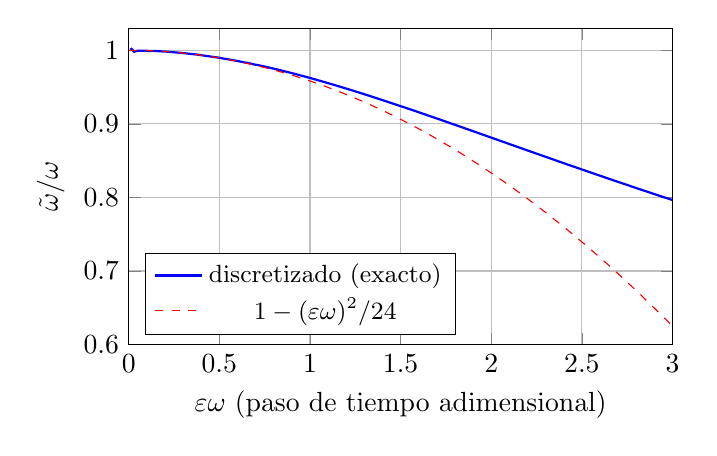
\begin{tikzpicture}
\begin{axis}[
    width=0.7\textwidth, height=5.6cm,
    xlabel={$\varepsilon\omega$ (paso de tiempo adimensional)},
    ylabel={$\tilde\omega/\omega$},
    xmin=0, xmax=3, ymin=0.6, ymax=1.03,
    grid=major, legend pos=south west, legend style={font=\small}]
\addplot[domain=0.01:3, samples=150, thick, blue]
    {ln(1+x^2/2+sqrt((1+x^2/2)^2-1))/x};
\addlegendentry{discretizado (exacto)}
\addplot[domain=0:3, samples=60, dashed, red] {1-x^2/24};
\addlegendentry{$1-(\varepsilon\omega)^2/24$}
\end{axis}
\end{tikzpicture}
\caption{Frecuencia efectiva del oscilador discretizado en función del paso de tiempo. Sirve para decidir cuántos pasos $N$ usar en una simulación.}
\label{fig:discret}
\end{figure}

\campo{Leer}
\F{10} \S2 (métodos: Metropolis--Hastings y estimadores) y ap.~B y D. Apoyo: \F{02} cap.~1, sección \textit{Numerical Treatment of Path Integrals}.

\campo{Preguntar a NotebookLM}
\begin{prompt}
Según \F{10}, ¿qué estimador de la energía del estado fundamental se usa en Path Integral Monte Carlo y cómo depende su error del número de pasos? Dame el algoritmo en pseudocódigo con referencia a la sección.
\end{prompt}

\campo{Ejercicio}
Programar (Python, unas 30 líneas) el PIMC del oscilador con $\hbar=m=\omega=1$ y obtener $E_0\approx0.5$ con error menor al $2\%$.

\campo{Autoevaluación}
¿Por qué este método no funciona directamente en tiempo real?

%----------------------------------------------------------------------
\sesion{10 --- Campo electromagnético y topología}{1 h}

\campo{Idea clave}
Con un potencial vector, $L\to L+\tfrac{e}{c}\dot{\mathbf x}\cdot\mathbf A$, cada camino gana la fase $\tfrac{e}{\hbar c}\int\mathbf A\cdot\dd\mathbf x$. Dos caminos que rodean un solenoide por lados opuestos difieren en $e\Phi/\hbar c$ aunque el campo magnético sea nulo por donde pasan: es el \textbf{efecto Aharonov--Bohm}. La fase depende solo de cuántas vueltas da el camino (topología). La misma idea explica por qué en 3D solo hay bosones y fermiones y en 2D pueden existir \textbf{anyones}, y por qué un monopolo magnético obligaría a cuantizar la carga (Dirac).

\campo{Leer}
\F{01} \S4 (\textit{Topology and Path Integrals}: Aharonov--Bohm, estadística, monopolos). Apoyo: \F{13} cap.~5; \F{06} \S18.

\campo{Preguntar a NotebookLM}
\begin{prompt}
Con \F{01} \S4, explica por qué en dos dimensiones pueden existir anyones y en tres no. Cita el argumento sobre el espacio de configuración de dos partículas idénticas.
\end{prompt}

\campo{Ejercicio}
Dibujar dos caminos alrededor de un solenoide y calcular su diferencia de fase. Deducir que el patrón de interferencia se desplaza periódicamente con $\Phi$, con periodo $hc/e$.

\campo{Autoevaluación}
¿Por qué la fase de Aharonov--Bohm no depende de la forma exacta del camino?

%----------------------------------------------------------------------
\sesion{11 --- Efecto túnel e instantones}{1 h}

\campo{Idea clave}
En tiempo imaginario el potencial se invierte ($V\to-V$ en la ecuación de movimiento euclídea). En un doble pozo, la trayectoria euclídea que va de un mínimo al otro, el \emph{instantón}, domina la amplitud de túnel, y el desdoblamiento de niveles resulta $\Delta E\propto e^{-S_{\text{inst}}/\hbar}$. Es un efecto no perturbativo que la teoría de perturbaciones no ve a ningún orden.

\campo{Leer}
\F{13} cap.~4 (\textit{Instantons}, \S4.2 doble pozo). Apoyo: \F{01} \S8 (\textit{Instantons in Quantum Mechanics}).

\campo{Preguntar a NotebookLM}
\begin{prompt}
Según \F{13} cap.~4, ¿cómo se obtiene el desdoblamiento de energía en el doble pozo con instantones? ¿Qué es el ``gas diluido de instantones''? Cita las ecuaciones.
\end{prompt}

\campo{Ejercicio}
Para $V=\lambda(x^2-a^2)^2$, encontrar la solución instantón $x(\tau)$ y su acción $S_{\text{inst}}$.

\campo{Autoevaluación}
¿Por qué $e^{-S_{\text{inst}}/\hbar}$ no se puede desarrollar en potencias de $\hbar$?

%----------------------------------------------------------------------
\sesion{12 --- Átomo de hidrógeno y puente a la teoría de campos}{1 h}

\campo{Idea clave}
\textbf{Hidrógeno (lectura guiada, 30 min).} El potencial de Coulomb $-e^2/r$ no se deja tratar por la discretización directa porque los caminos ``caen'' al origen. Duru y Kleinert (1979) lo resolvieron cambiando el tiempo, $\dd t=r\,\dd s$, y las coordenadas (Kustaanheimo--Stiefel): el problema se convierte en un oscilador armónico en 4D, que ya se sabe resolver.

\textbf{Campos (30 min).} Sustituyendo $x(t)\to\phi(\mathbf x,t)$, la misma construcción da la integral funcional de una teoría de campos, $Z[J]=\int\mathcal D\phi\,e^{iS[\phi]/\hbar+i\int J\phi}$, y las funciones de correlación salen de derivar respecto de $J$.

\campo{Leer}
\F{03} \S III.5 (\textit{The Coulomb Potential}); \F{04}, sección \textit{Hydrogen Atom}; para la historia, \F{14}. Campos: \F{07} \S3--4; \F{12} \S3.6 (funcional generatriz).

\campo{Preguntar a NotebookLM}
\begin{prompt}
Compara cómo resuelven el átomo de hidrógeno \F{03} y \F{04}: ¿qué transformación usa cada uno y qué interpretación le da \F{04} como gravedad cuántica en una dimensión?
\end{prompt}

\campo{Autoevaluación}
Explicar en cinco líneas por qué el hidrógeno fue un problema abierto de la formulación de Feynman hasta 1979.

%======================================================================
\section{Autoevaluación final}
\label{sec:final}

Hacerla sin fuentes ni IA (30 min, fuera de las 12 h). Si falla una pregunta, se repite la sesión indicada.

\begin{enumerate}
    \item Deducir la integral de camino desde $\langle x_b|e^{-i\hat HT/\hbar}|x_a\rangle$. \hfill (S3)
    \item Calcular $K_0$ y comprobar sus dimensiones y su límite $T\to0$. \hfill (S4)
    \item Explicar por qué $\hbar\to0$ selecciona la trayectoria clásica. \hfill (S7)
    \item Escribir $Z(\beta)$ como integral de camino y decir por qué los caminos son cerrados. \hfill (S8)
    \item Explicar el efecto Aharonov--Bohm con dos caminos. \hfill (S10)
    \item Pedir a NotebookLM: \emph{``Genera 10 preguntas de opción múltiple sobre las sesiones 1--8, cada una con la fuente y la sección de donde sale la respuesta''}, y verificar cada respuesta en la fuente, no en la IA.
\end{enumerate}

%======================================================================
\appendix
\section{Anexo: preparación del cuaderno y auditoría de la IA}

\textbf{Fuentes.} El cuaderno del profesor tiene 16 PDF con nombres poco informativos (\texttt{9302097v1.pdf}, \dots). Los títulos y autores se sacaron pidiéndoselos al propio cuaderno, y los identificadores de arXiv se comprobaron contra arXiv. Había un archivo duplicado (MacKenzie), así que son 15 obras.

\textbf{Por qué se pasaron a Markdown.} El texto que NotebookLM extrae de los PDF rompe las ecuaciones: en \F{06}, $S=\int L(x,\dot x)\,\dd t$ aparece como símbolos sueltos en líneas distintas. Pasar los PDF por otro extractor de texto no lo arregla, porque es el mismo procedimiento, y en los PDF escaneados no hay texto que extraer. Por eso:
\begin{itemize}
    \item \F{01}, \F{02} y \F{04} se convirtieron desde el código \LaTeX{} original de arXiv, con las ecuaciones tal como las escribió el autor;
    \item el resto se transcribió con IA con visión (Claude), leyendo cada página como imagen;
    \item \F{08} (1641 páginas) se deja en PDF; \F{14} y \F{15} tienen derechos de autor y se consultan en la copia del curso;
    \item incidencias: \F{05} tiene sin transcribir las pp.~28--30, que remiten al PDF; en \F{10} el código C++ se resumió.
\end{itemize}

\textbf{Errores de la IA detectados.}
\begin{enumerate}
    \item Al pedirle a Gemini las 16 fuentes, devolvió una lista en la que solo cinco coincidían con los archivos reales. Las otras once eran referencias conocidas del tema (Feynman 1948, Dirac 1933, Wiener, Gelfand--Yaglom, etc.) que no estaban en el cuaderno. Respondió a ``qué se suele leer sobre esto'' y no a ``qué hay aquí''. Por eso todos los prompts de la guía exigen citar la fuente y la ecuación.
    \item Metadatos: el año de \F{02} es 2012 (v1) o 2017 (v4, el archivo usado); el de \F{03} es 1992 (texto) o 1993 (envío a arXiv). Se usan las fechas del archivo.
    \item Las ecuaciones transcritas por IA llevan en su cabecera el aviso de revisar las críticas contra el PDF. Las más densas señaladas son la ec.~(27) de \F{11} y las del capítulo de instantones de \F{13}.
\end{enumerate}
